\documentclass{article}
%\usepackage[utf8]{inputenc}
\usepackage[utf8]{vietnam}
\usepackage{amsmath,amsxtra,amssymb,latexsym, amscd,amsthm}
\usepackage{mathtools}
\usepackage{graphicx}
\usepackage{wrapfig}
\usepackage{blindtext}
\usepackage{csquotes}


\newcommand{\norm}[1]{\left\lVert#1\right\rVert}
\newcommand{\twonorm}[1]{\left\lVert#1\right\rVert_{2}}
\renewcommand\qedsymbol{$\blacksquare$}
\newtheorem*{theorem}{Theorem}
\newtheorem*{axiom}{Axiom}

\title{$p\,$-norm of matrices}
\author{phunc20}
\date{\today}


\begin{document}
\theoremstyle{definition}
\newtheorem{Spiel}{Vd}[section]


\maketitle
\section{Động cơ}
%Tại sao người ta lại nghĩ đến định nghĩa $\Vert A \Vert := \sup_{\bold{x} \ne \bold{0}} \frac{A\bold{x}}{\Vert \bold{x} \Vert}$
%Tại sao người ta lại nghĩ đến định nghĩa $\Vert A \Vert \mathrel{\mathop:}= \sup_{\bold{x} \ne \bold{0}} \frac{A\bold{x}}{\Vert \bold{x} \Vert}$
%Tại sao người ta lại nghĩ đến định nghĩa $\Vert A \Vert \coloneqq \sup_{\bold{x} \ne \bold{0}} \frac{A\bold{x}}{\Vert \bold{x} \Vert}$
Tại sao người ta lại nghĩ đến định nghĩa norm của một ma trận $A \in M_{m,n}(\mathbb{C})$
$$\norm{A} \,\,\coloneqq\!\! \sup_{\mathbf{x} \,\in\, {\mathbb{C}^{n} \setminus \{\mathbf{0}\}}} \frac{\norm{A\mathbf{x}}}{\norm{\mathbf{x}}}\;$$
như thế này?

\textbf{Rmk.} Why we choose to not specify exactly which norm above?

\textbf{Rmk2.} Cho dù mình viết $\mathbb{C}^n$ bạn đọc cũng có thể suy nghĩ trong $\mathbb{R}^n$.

\section{Ý tưởng}
Bây giờ giả bộ như chúng ta không biết về sự tồn tại của định nghĩa này, và chúng ta cùng đi tìm một định nghĩa hợp lý
cho norm của một ma trận. Các norm $\norm{A\mathbf{x}}$ va $\norm{\mathbf{x}}$ đã được định nghĩa rõ rằng, lúc này  mình sẽ tự hỏi
\begin{displayquote}
chúng ta có thể định nghĩa ra $\norm{A}$ sao cho $\norm{A\mathbf{x}} \stackrel{?}{=} \norm{A}\cdot\norm{\mathbf{x}}$ không?
\end{displayquote}

%Tiếp theo chúng ta sẽ đi kiểm ví dụ ngược/trốn lại cái đẳng thức ở trên. Nếu kiểm không được mình sẽ đi chứng minh nó.
Một counter-example có thể hướng dẫn chúng ta:
%\begin{proof}
\begin{Spiel}
  %Consider the following matrix and vectors with the standard $2$-norm in $\mathbb{R}$\\
	Xét ma trận $A$ và vectơ $\mathbf{x_1}, \mathbf{x_2}$ như sau
  $$
    A = \begin{pmatrix}
    	3 &  5 \\
    	4 & 12 \\
    \end{pmatrix},\;
    \mathbf{x_1} = \begin{pmatrix} 1 \\ 0 \end{pmatrix},\;
    \mathbf{x_2} = \begin{pmatrix} 0 \\ 1 \end{pmatrix}.
  $$
  %with the standard $2$-norm in $\mathbb{R}$
  Với cái $2$-norm quen thuộc trong $\mathbb{R}^2$, chúng ta có
  $$
	  \begin{aligned}
			%% Cannot \small neither \tiny in math mode
			%\norm{\mathbf{x_1}}_{\small 2} = 1, \twonorm{\mathbf{x_2}} = 1
			%\norm{\mathbf{x_1}}_{\tiny 2} = 1, \twonorm{\mathbf{x_2}} = 1
			%& \norm{\mathbf{x_1}}_{2} = 1,\; \twonorm{\mathbf{x_2}} = 1, \\
			& \norm{\mathbf{x_1}}_{2} = 1,\; \twonorm{\mathbf{x_2}} = 1, \nonumber \\
			& \norm{A \mathbf{x_1}}_{2} = \norm{\begin{pmatrix} 3 \\ 4 \end{pmatrix}}_{2} = 5, \\
			%& \begin{equation}
			%	  \norm{A \mathbf{x_1}}_{2} = \norm{\begin{pmatrix} 3 \\ 4 \end{pmatrix}}_{2} = 5,
      %  \end{equation} \\
			& \norm{A \mathbf{x_2}}_{2} = \norm{\begin{pmatrix} 5 \\ 12 \end{pmatrix}}_{2} = 13. \\
	  \end{aligned}
  $$
	Từ ví dụ này chúng ta có thể nhìn ra $\norm{A\mathbf{x}} \stackrel{?}{=} \norm{A}\cdot\norm{\mathbf{x}}$ \textbf{không khá thi}. Bởi vì nếu như đẳng thức có thật, thì 
  $$
	  \begin{aligned}
			\norm{A \mathbf{x_1}}_{2} = 5 &\implies \norm{A}_{2} = 5 \\
			\norm{A \mathbf{x_2}}_{2} = 13 &\implies \norm{A}_{2} = 13 \\
			\qquad\qquad\qquad \rightarrow\!\leftarrow\; &\text{(Contradiction)}
	  \end{aligned}
  $$
  \hfill\qedsymbol
\end{Spiel}
%\end{proof}

Nếu vậy sẽ rất hợp lý cho chúng ta chuyển sang một mục tiêu yếu hơn, đó là
$$
  \begin{aligned}
    \norm{A\mathbf{x}} \stackrel{?}{\le} \norm{A}\cdot\norm{\mathbf{x}} \quad\forall\;\; \mathbf{x} \in \mathbb{C}^n \\
		\\
		\text{tương đương với} \\
		\\
		\norm{A} \stackrel{?}{\ge}  \frac{\norm{A\mathbf{x}}}{\norm{\mathbf{x}}}  \quad\forall\;\; \mathbf{x} \ne \mathbf{0}. \\
  \end{aligned}
$$
Chúng ta đã có thể nhận ra hình dáng của định nghĩa \textit{bí ấn} ban đầu.

Nhắc lại $\sup S$ của một tập $S \subset \mathbb{R}$ tiếng Anh được gọi là \textit{least upper bound}, tức là con số chặn trên nhỏ nhất.
Chúng ta dĩ nhiên sẽ hỏi:
Tập $\left\{\frac{\norm{A\mathbf{x}}}{\norm{\mathbf{x}}} \;|\; \mathbf{x} \in \mathbb{C}^n \setminus \mathbf{0}\right\}$ có bị chặn ở trên không?


Quan sát hàm $\mathbf{x} \mapsto \frac{\norm{A\mathbf{x}}}{\norm{\mathbf{x}}},\; \mathbf{x} \in \mathbb{C}^n \setminus \{\mathbf{0}\}.$ Chúng ta có

$$
%\begin{equation}
	%\forall\; c \in \mathbb{R}^{+} \setminus \{0\},
	\forall\; c \in \mathbb{R}^{+},\;
	c\mathbf{x} \mapsto \frac{\norm{A(c\mathbf{x})}}{\norm{c\mathbf{x}}} = 
  \frac{c\norm{A\mathbf{x}}}{c\norm{\mathbf{x}}} =
  \frac{\norm{A\mathbf{x}}}{\norm{\mathbf{x}}}.
%\end{equation}
$$

Từ cái này chúng ta rút ra một kết quả nhỏ, đó là

$$
  % Set LHS of an equation
  \left\{ \frac{\norm{A\mathbf{x}}}{\norm{\mathbf{x}}} \vert\;
	\mathbf{x} \in \mathbb{C}^n \setminus \{\mathbf{0}\} \right\} =
  % Set RHS of an equation
  \left\{ \frac{\norm{A\mathbf{x}}}{\norm{\mathbf{x}}} \vert\;
	\mathbf{x} \in \mathbb{C}^n \text{and} \norm{\mathbf{x}} = 1 \right\}.
	%\{ \frac{\norm{A\mathbf{x}}}{\norm{\mathbf{x}}} |\;
	%\mathbf{x} \in \mathbb{C}^n \text{and} \norm{\mathbf{x}} = 1 \} 
$$

Điều này có nghĩa là
\textbf{
	chúng ta chỉ cần chứng minh rằng hàm
  $\mathbf{x} \mapsto \frac{\norm{A\mathbf{x}}}{\norm{\mathbf{x}}}$
	được chặn ở trên khi $\mathbf{x}$ thuộc về unit circle
	$\left\{\mathbf{x} \in \mathbb{C}^n \vert \norm{\mathbf{x}} = 1\right\}$
}.

Để chứng minh điều này, tôi sẽ sử dụng một kết quả nổi tiếng và cơ bản trong toán phân tích. [Rmk. nếu sau này tôi biết về một phương pháp nào đó còn đơn giản hơn nữa thì tôi sẽ lại đây update; nếu các bạn nào chưa có học qua về cái kết quả này và thắc mắc về nó, có thể thăm khảo blahblahblah] 

\begin{theorem}
If $f: K \subset \mathbb{C}^n \to \mathbb{R}$ is continuous and $K$ is closed and bounded, (i.e. compact)
then $f(K)$ is also closed and bounded.
\end{theorem}

If the norm $\norm{\cdot}$ is a continuous function (in particular, all the $p$-norms are continuous), then our function $\mathbf{x} \mapsto \frac{\norm{A\mathbf{x}}}{\norm{\mathbf{x}}}$ is clearly continuous and the unit circle is closed and bounded, whence the set in question is bounded (both above and below).


\begin{axiom}
	If $\,\forall A \subset \mathbb{R}$ that is bounded above, there exists $a \in \mathbb{R}$ s.t. $\forall\, \text{upper bound}\;\, u\; \text{of}\; A$ we have $a \le u$; in other words, the \textit{least upper bound} of $A$ exists.
\end{axiom}


Tổng lại, chúng ta đã nhận ra:\newline
với đa số norm, it is legitimate to define 
$$
  \norm{A}
	\,\,\coloneqq\!\!
	\sup_{\mathbf{x} \,\in\, {\mathbb{C}^{n} \setminus \{\mathbf{0}\}}} \frac{\norm{A\mathbf{x}}}{\norm{\mathbf{x}}}\;
	= 
	%\sup_{\mathbf{x} \,\in\, {\mathbb{C}^{n} \setminus \{\mathbf{0}\}}} \norm{A\mathbf{x}}
	\sup_{\left\{\mathbf{x} \in \mathbb{C}^n \vert \norm{\mathbf{x}} = 1\right\}} \norm{A\mathbf{x}}
$$













\begin{wrapfigure}{p}{0.5\textwidth}
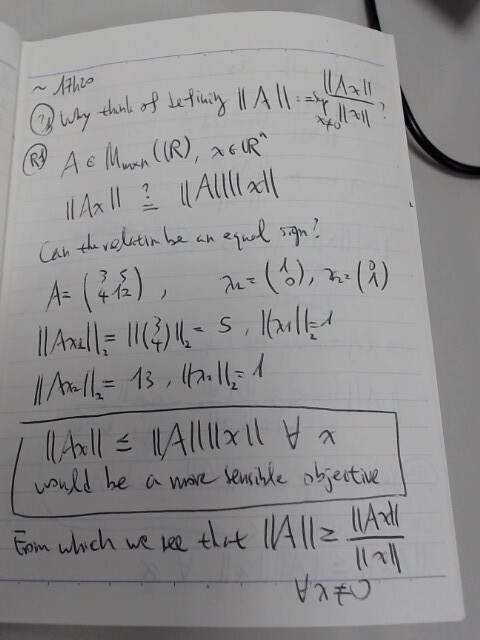
\includegraphics[width=0.4\textwidth]{01-motivation.jpg}
%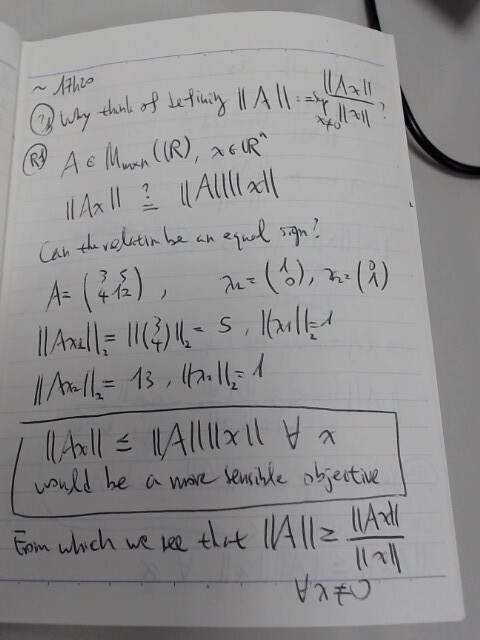
\includegraphics[width=2.5cm]{01-motivation.jpg}
%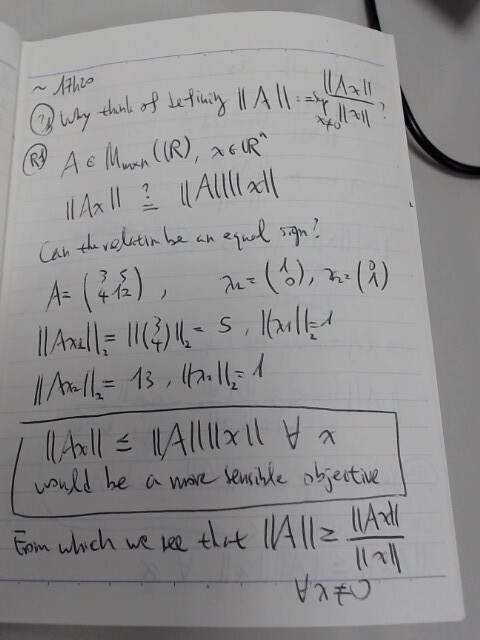
\includegraphics{01-motivation.jpg}
\end{wrapfigure}

\begin{wrapfigure}{h}{0.5\textwidth}
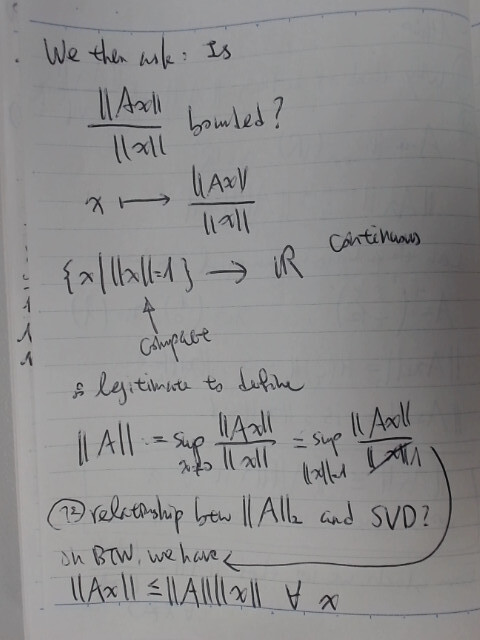
\includegraphics[width=0.4\textwidth]{02-moti_cont.jpg}
\end{wrapfigure}


%\blindtext

%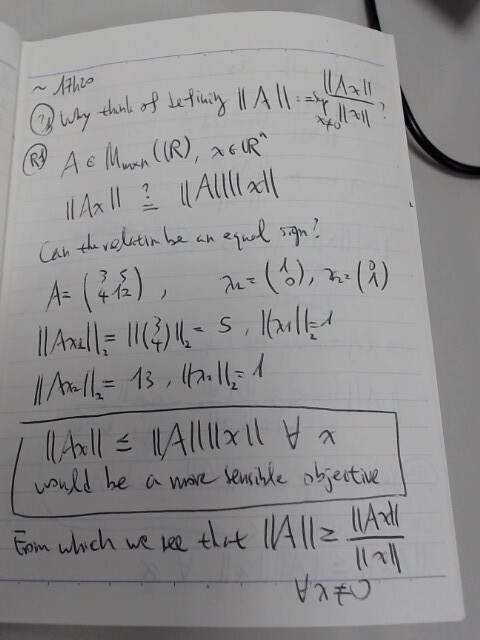
\includegraphics[width=0.7\textwidth]{01-motivation.jpg}
%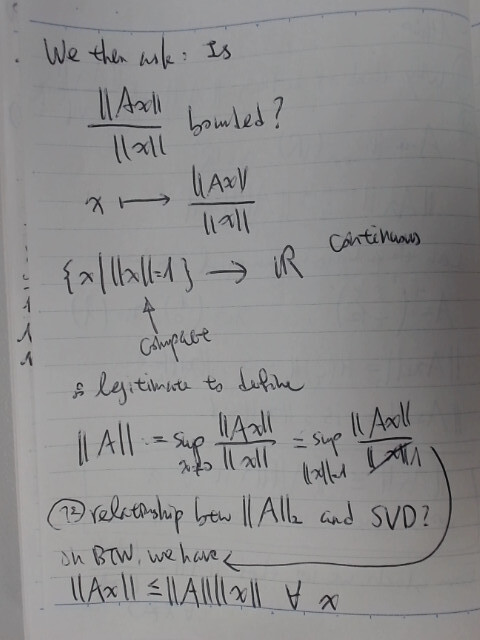
\includegraphics[width=0.7\textwidth]{02-moti_cont.jpg}
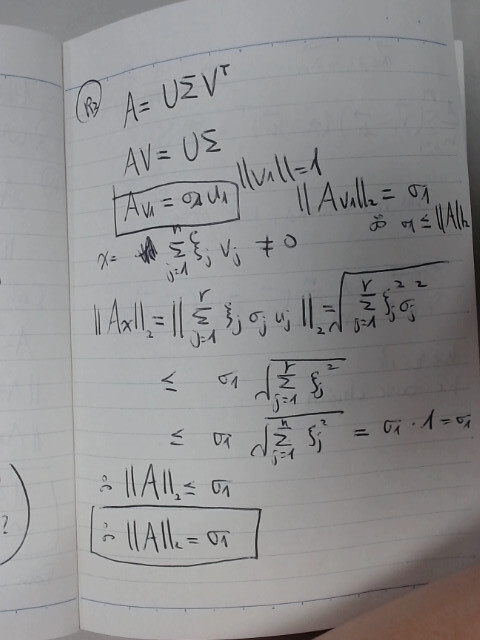
\includegraphics[width=0.4\textwidth]{03-2norm_and_singular_value.jpg}
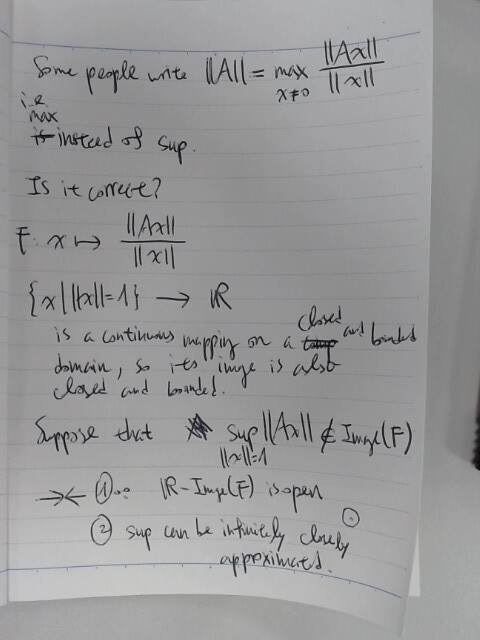
\includegraphics[width=0.4\textwidth]{04-max_instead.jpg}

\end{document}





